    
        \subsubsection{Logical Data Model}

            \begin{figure}[H]
                \centering
                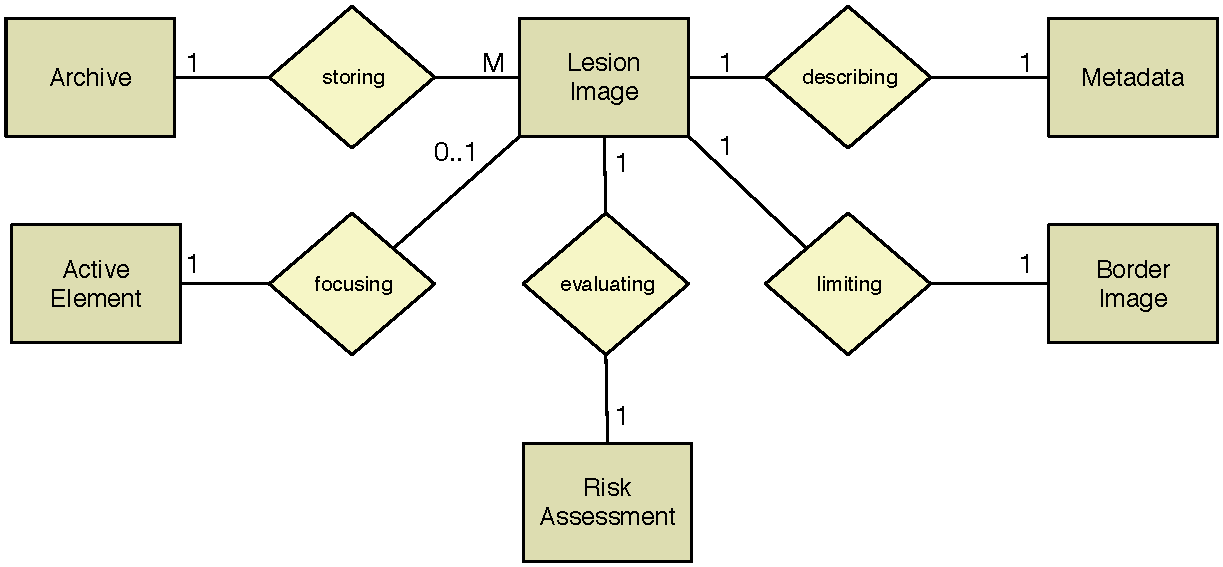
\includegraphics[width=\textwidth]{assets/requirements/EntRel.pdf}
                \caption{Patial data model of the Melanoma Detection App}
                \label{fig:partial_data_model}
            \end{figure}


        \subsubsection{Data Dictionary}

                \begin{longtable}[H]{ | l | p{3.0cm} | p{2.5cm} | p{1.0cm} | p{2.5cm} | }

                    \hline
                    \textbf{Data element} & \textbf{Description} & \textbf{Componsition or data type} & \textbf{Length} & \textbf{Values} \\ \hline

                    \hypertarget{lesion_image}{Lesion Image} & reference to the captured image &

                        \specialcell[t]{Image ID
                           \\ + File Path
                           \\ + Creation Date
                        }

                     & & \\ \hline

                    Image ID & unique identifier for an image &
                    integer & 11 & system-generated sequential integer beginning with 1 \\ \hline

                    File Path & location of a file on the file system &
                    string & 256 &  \\ \hline

                    Creation Date & date and time that a file was created &
                    DDMMYYYYHHSS &  &  \\ \hline

                    Metadata & information describing the lesion and it's location &

                        \specialcell[t]{\hyperlink{lesion_image}{Lesion Image}
                           \\ + Lesion Description
                           \\ + Lesion Location
                        }

                     & & \\ \hline

                    Lesion Description & User defined text that describes the lesion &
                    alphanumeric &  &  \\ \hline

                    Lesion Location & information describing the lesion location on the body &

                        \specialcell[t]{\hyperlink{lesion_image}{Lesion Image}
                           \\ + Body Location ID
                           \\ + X Coordinate
                           \\ + Y Coordinate
                        }

                     & & \\ \hline


                    Body Location ID & id of a region on the body &
                    integer & 2 &

                        \specialcell[t]{
                            1 : Head Front \\
                            2 : Torso Front \\
                            3 : Right Upper Arm \\
                            4 : Left Upper Arm \\
                            5 : Right Forearm \\
                            6 : Left Forearm \\

                        }

                     \\ \hline

                    X Coordinate & x coordinate of the lesion in the region specified by the body location id &
                    integer & 128 &  \\ \hline

                    Y Coordinate & y coordinate of the lesion in the region specified by the body location id &
                    integer & 128 &  \\ \hline

                    Border Image & data that defines the outline of the lesion area &

                        \specialcell[t]{\hyperlink{lesion_image}{Lesion Image}
                           \\ + File Path
                           \\ + Creation Date
                        }

                     & & \\ \hline

                    Risk Assessment &  &

                        \specialcell[t]{\hyperlink{lesion_image}{Lesion Image}
                            \\ + Assessment Date
                            \\ + Version Number
                            \\ + SFA Major
                            \\ + SFA Minor
                            \\ + Border Irregularity
                            \\ + Color Score
                            \\ + \hyperlink{tds_score}{TDS Score}
                        }

                    & & \\ \hline

                    Assessment Date & date and time that the risk assessment was calculated &
                    DDMMYYYYHHSS &  &  \\ \hline

                    Version Number & version number of the risk assessment service software &
                    integer & 4 &  \\ \hline

                    SFA Major & measure of symmetry of the lesions major axis &
                    integer & 3 & 0 - 360 \\ \hline

                    SFA Minor & measure of symmetry of the lesions minor axis &
                    integer & 3 & 0 - 360 \\ \hline

                    Border Irregularity & measure of irregulatiry of the lesion's border &
                    integer & 1 & 0 - 8 \\ \hline

                    Color Score & number of specific colors found in the lesion's image &
                    integer & 1 & 0 - 8 \\ \hline

                    \hypertarget{tds_score}{TDS Score} & weighted linear combination of the image features summarizing the risk assessment  &
                    float &  & 1 - 8.9 \\ \hline

                    Archive &  &

                        \specialcell[t]{Archive ID
                            \\ + \hyperlink{lesion_image}{Lesion Image}
                            \\ + Metadata
                            \\ + Border
                            \\ + Risk Assessment
                            \\ + Archive Date
                        }

                     & & \\ \hline


                    Color Score & number of specific colors found in the lesion's image &
                    integer & 1 & 0 - 8 \\ \hline

                \end{longtable}


        \subsubsection{Data analysis}
            \paragraph{CRUD Matrix}

                A CRUD ( Create, Read, Update, Delete ) matrix can highlight which use cases interact with which data entities and in which way. Every entity that is read or deleted also needs to be created somewhere. The CRUD matrix in figure \ref{fig:crud} shows that this is the case.

                \begin{figure}[H]
                    \centering
                    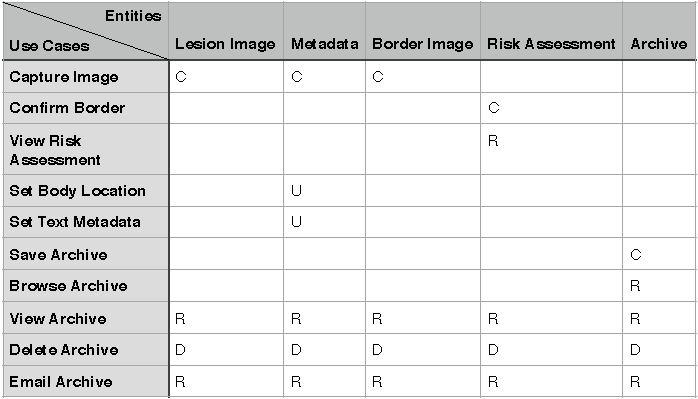
\includegraphics[width=\textwidth]{assets/requirements/CRUD.pdf}
                    \caption{CRUD matrix for Melanoma Detection App}
                    \label{fig:crud}
                \end{figure}

        \subsubsection{Reports}
            \paragraph{Email Report}
                When the Smartphone User chooses to send an archive as an email, the data must be flattened into a format that is email compatible. The body of the email will be an html document that displays the lesion image, the calculated border, the risk assessment data and the associated metadata.


